\section{Architecture}

Figure \ref{fig:arch_01} illustrates a high level overview of the distributed audio proessing environment. The user of the system interacts with the audio production software running on the host CPU and can choose to activate an audio processing plugin on a specific audio track. A single audio plugin might contain one or several individual processors. Processor that are enabled for distributed processing will search for a corresponding processor on a network SBC device.

The devices are networked via gigabit ethernet. It is assumed that the network is not being used for any other significant traffic.

\begin{figure}[H]
    \centering
    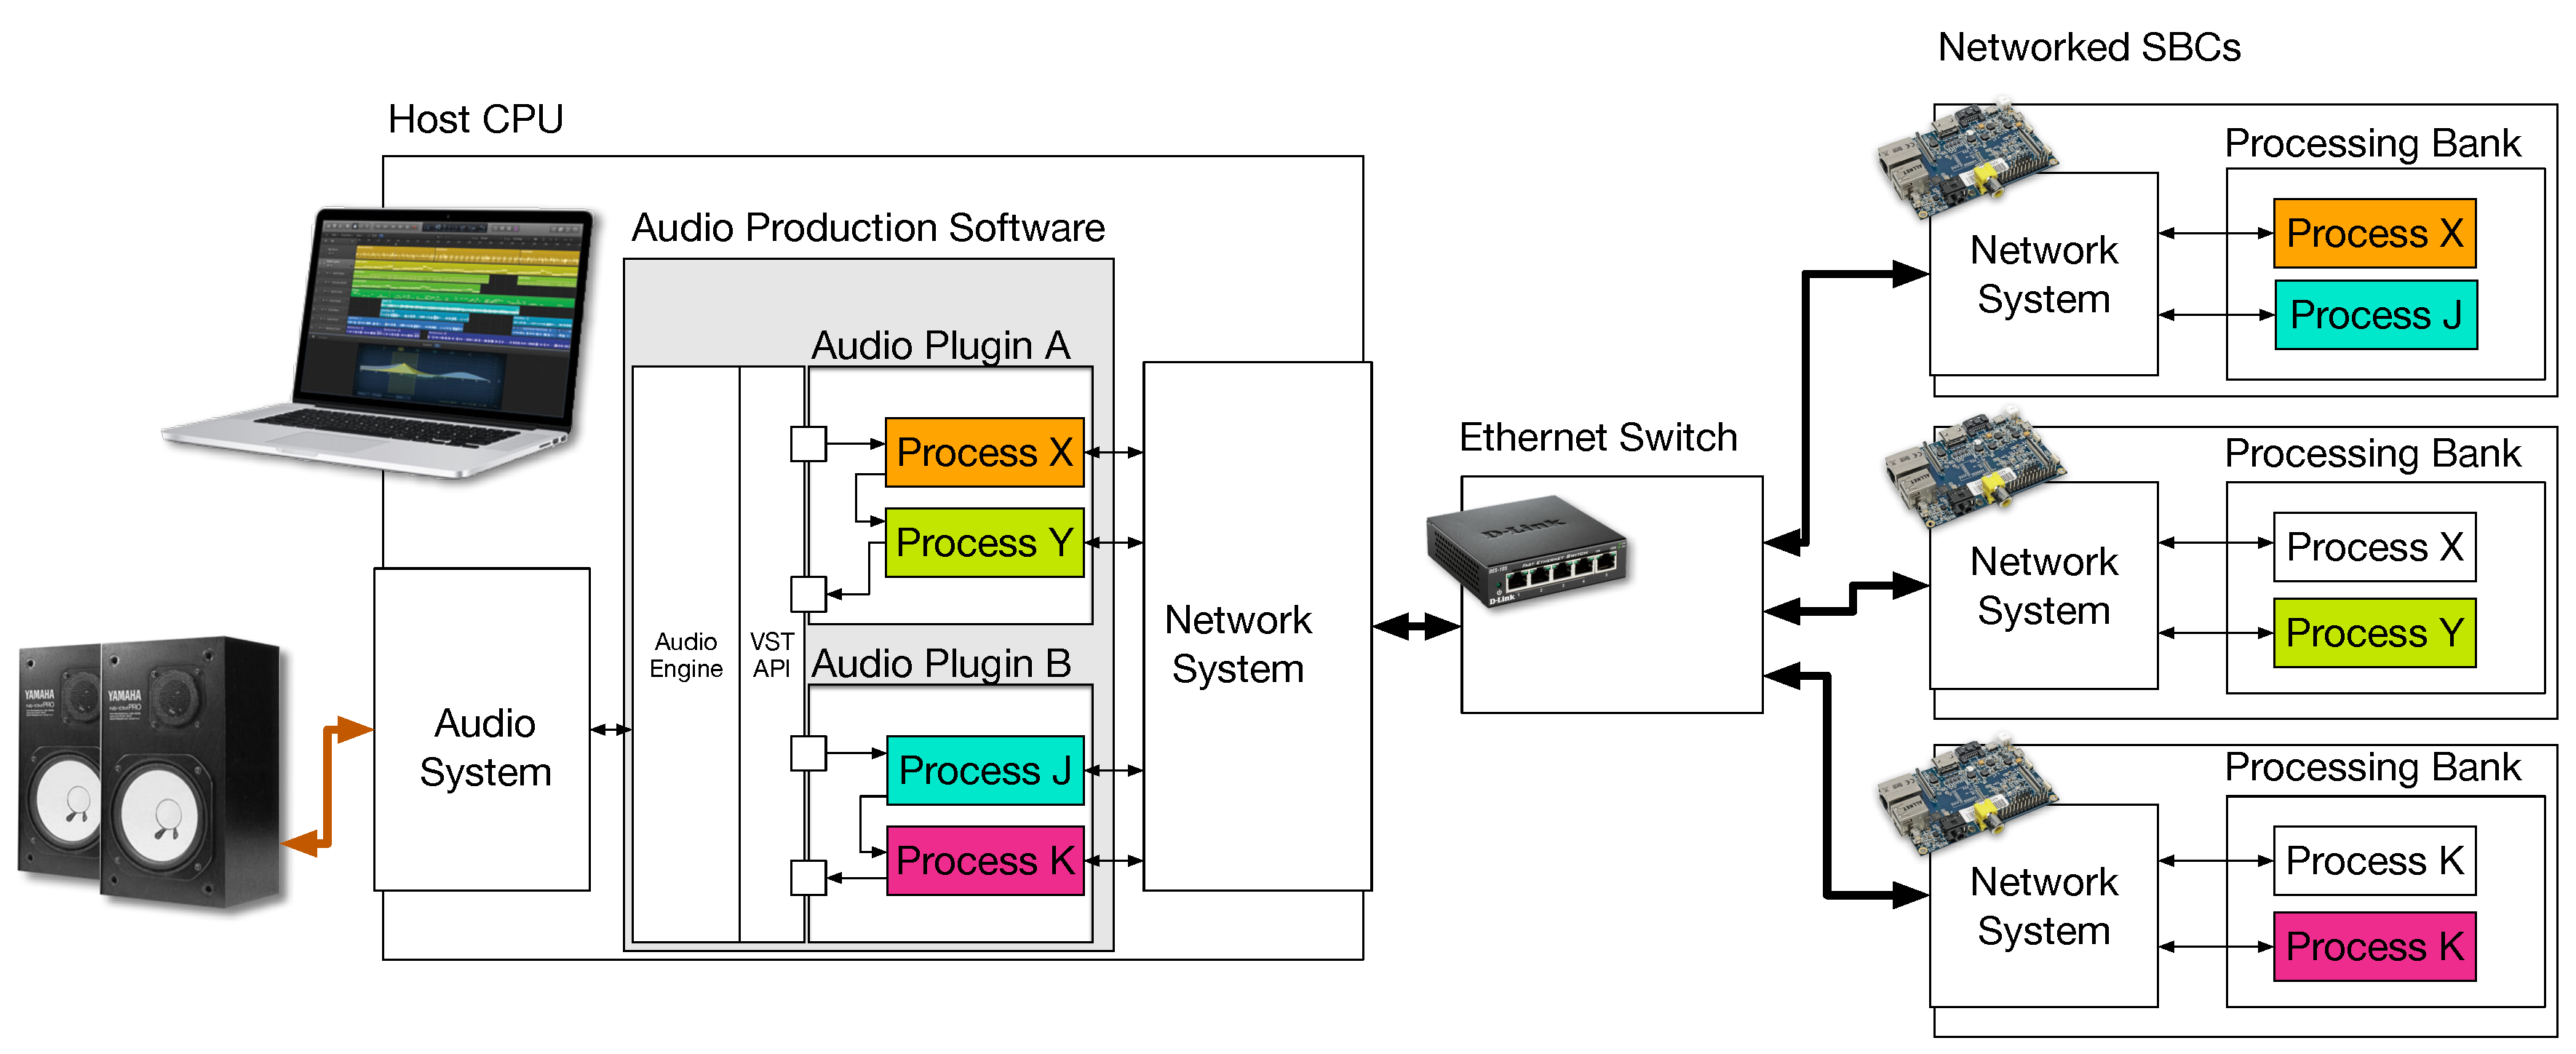
\includegraphics[width=\textwidth]{assets/architecture_01.pdf}
    \caption{Architectural Overview}
    \label{fig:arch_01}
\end{figure}

\subsection{Host CPU}

Figure \ref{fig:arch_02} zooms in on the components involved in realtime audio on the CPU. The audio hardware needs to provide a constant stream of data to it's digital to analog converters. It does this by periodically polling the operating system for a buffer of data via hardware interrupts. The requested buffer size can be as small as 32 samples and the polling intervals less than 1 ms depending on the hardware and drivers.

The operating system provides an abstraction layer in the form of an API to the application software. This gives the application software a single API to interface with regardless of the brand of audio hardware and drivers installed.

The VST API is another abstraction layer that offers a unified interface for plugin vendors to develop against. But VST is not the only plugin API. The Juce library offers it's own plugin API to develop against, which is simpler and abstracts away the differences between other plugin APIs.

The requests for data, manifested as interrupts triggered by the audio hardware, are passed on through the system to the audio production software by means of callbacks that the application has registered with the system. The audio production software in turn polls all the active plugins for data through thier defined VST callback functions.

\begin{figure}[H]
    \centering
    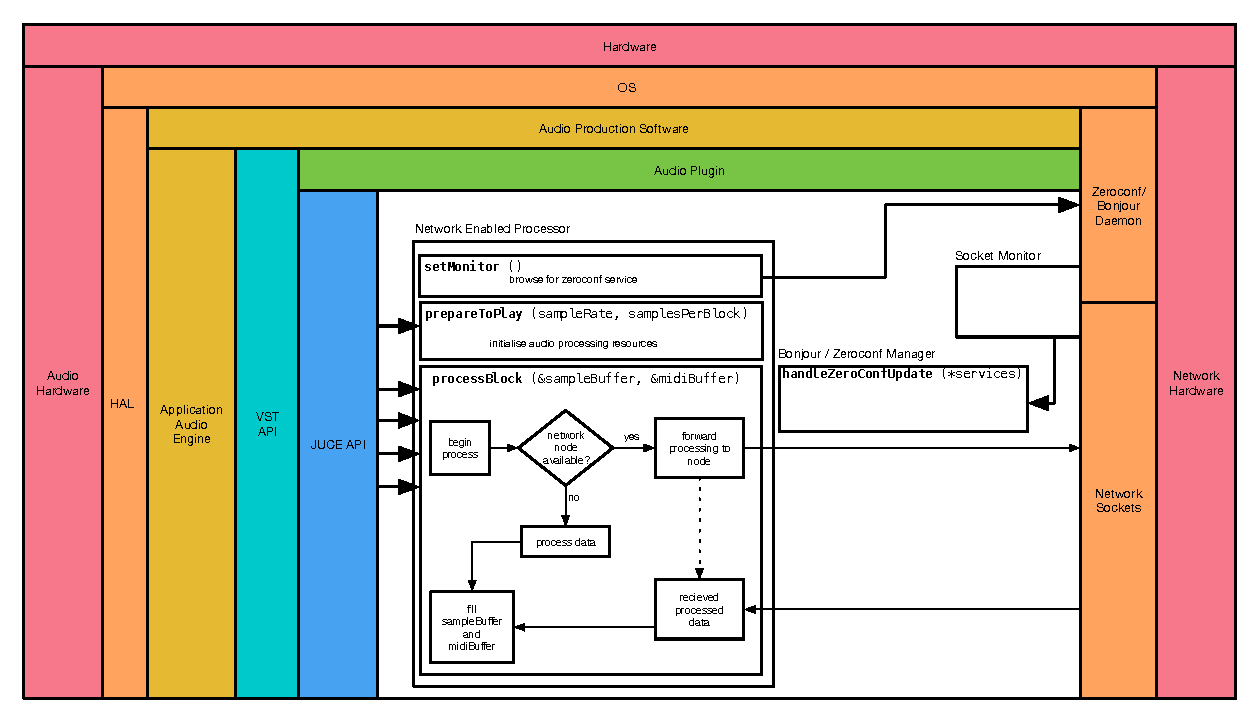
\includegraphics[width=\textwidth]{assets/architecture_02.pdf}
    \caption{Host CPU Overview}
    \label{fig:arch_02}
\end{figure}

The plugin implemented for this project has several network enabled processors, in figure \ref{fig:arch_02} only one is shown as an example. When the plugin the instanciated by the host software, it in turn instanciates each of it's processors. The processors in turn immediately calls the operating system's Bonjour / Zeroconf daemon with a request to browse the network for a specific service corresponding to a matching processor node. The request includes a socket by which the daemon will notify the processor of machtes it has found.

The Bonjour / Zeroconf daemon notifies the audio plugin by means of the socket, at which point the plugin's Bonjour / Zeroconf manager scans through the list of matching services to find on that is available. The plugins activeNode member is then set to that matching network service.

When a request for audio data is passed from the audio production software to the plugin, it does so by calling the processBlock function of the plugin. The plugin in turn calls the processBlock of each of its processors. In figure \ref{fig:arch_02} this is simplified showing only the processBlock of a single processor. The processBlock function is given a reference to the current audio buffer and midi buffer to process. The audio buffer contains the individual samples for each channel to be processed as float values. The midi buffer contains performance data regarding the timing and pitch of notes to be played.

Within the process block the processor checks if a activeNode is available. If so it immediately forwards the buffers of audio and midi as well as it's own state information to the activeNode and awaits the response. When the response arrived the data is copied back to the buffers and the function is ended.

\subsection{Networked SBCs}

\begin{figure}[H]
    \centering
    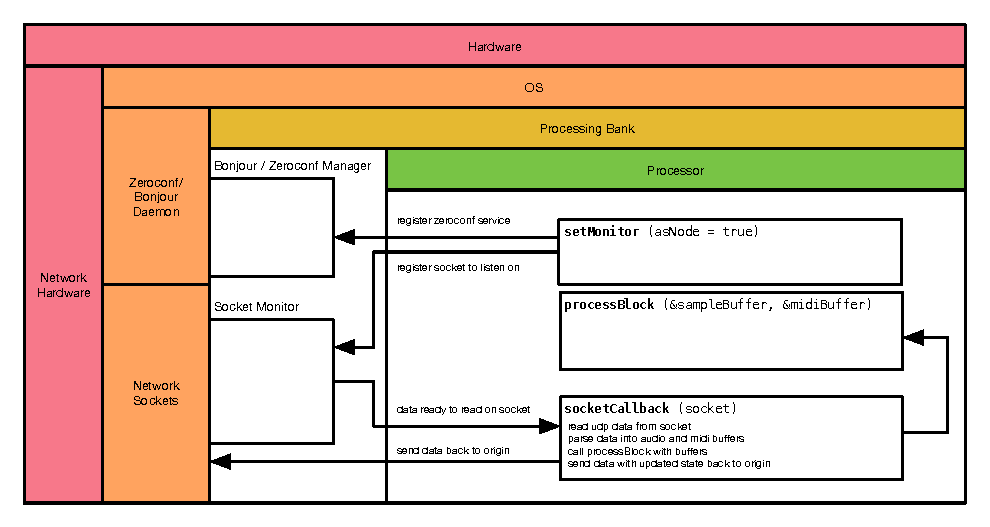
\includegraphics[width=\textwidth]{assets/architecture_03.pdf}
    \caption{SBC Processor Overview}
    \label{fig:arch_03}
\end{figure}
